\chapter{Glaze Problems}
Anybody with even a little experience with glazes will realize that problems 
often arise. Knowing what to do about them requires a lot of experience, and 
even expert glazers often find it difficult to establish the source of a 
problem.
%-------------------------------------------------------------------------------
\section{Introduction to Glaze Problems}
It is one thing to develop a nice glaze but quite another to keep it working. 
One potter may want a glaze that crazes, whereas another wants his glaze to be 
craze-free. A glaze fault may not mean that the glaze is ugly, just that it 
reacts differently and does not look like the desired effect.

When a glaze suddenly starts to react differently from what we want, we call it 
a glaze fault. Solving the problem is seldom easy, and usually several factors 
are involved. The first thing to check is what changes have occurred since the 
glaze last worked without problems. 

The following things should be checked:
%-------------------------------------------------------------------------------
\begin{itemize}
\item Was the right recipe used and were the materials weighed out correctly? 
(Always use batch cards for glaze weighing).
\item Were the right raw materials used? Was there any chance of mistaking one 
material for another? Was the labeling of materials in stock correct?
\item Have new raw materials or a new frit batch been used since the last 
fault-free glaze batch was produced? If so, check if the new material is 
different from the original material in stock.
\item Has the body been changed in any way? For example: new preparation 
method, change of clay material, change of body recipe, higher or lower biscuit 
firing?
\item Was the preparation of the glaze done as usual? For example: same ball 
milling time, same screening, same specific gravity of glaze slip?
\item Was there any change in glaze application and were the products clean and 
dust-free before application?
\item Were there changes in the kiln setting? Was the glazed ware dry before 
firing started? Were there any changes in fuel, firing schedule, firing 
atmosphere (reducing/oxidizing) and was the correct top temperature reached 
(setting of cones, draw trials) ?
\end{itemize}
%-------------------------------------------------------------------------------
Once we know which conditions have changed, we may already be close to 
establishing what caused the glaze problem. The following trouble-shooting 
lists may be helpful to find solutions to the problem.
%-------------------------------------------------------------------------------
\section{Troubleshooting Checklist}
%-------------------------------------------------------------------------------
\subsection{Glaze--Slip Problems}
%-------------------------------------------------------------------------------
\subsubsection{The glaze or part of the glaze settles too fast in the bucket.}
Causes
%-------------------------------------------------------------------------------
\begin{itemize}
\item High amount of frit in the glaze.
\item Glaze materials too coarse.
\item Water content of glaze slip too high.
\item Ball milling time was too short.
\item Too little clay in the slip.
\item Metal buckets cause fast settling.
\end{itemize}
%-------------------------------------------------------------------------------
Solutions
%-------------------------------------------------------------------------------
\begin{itemize}
\item Add 5--10\% plastic clay or 0.5--2\% bentonite.
\item Reduce amount of frit by removing some of the insoluble materials from 
the frit recipe and adding these to the glaze batch instead.
\item Longer ball milling of glaze materials.
\item Add a small amount of vinegar (acetic acid) to the glaze.
\item Use plastic buckets or wooden containers.
\end{itemize}
%-------------------------------------------------------------------------------
\subsubsection{Glaze slip is too thin, low viscosity.}
Causes
%-------------------------------------------------------------------------------
\begin{itemize}
  \item Water content too high.
  \item Alkali materials from frit or feldspar have been dissolved in the 
  water, so the slip is deflocculated.
\end{itemize}
%-------------------------------------------------------------------------------
Solutions
%-------------------------------------------------------------------------------
\begin{itemize}
  \item Let the glaze stand for a day and decant the clear water off the top. 
  Because some materials may be removed with the water, it is better to allow 
  excess water to evaporate.
  \item Add flocculant (magnesium sulfate, calcium chloride), but only if the 
  ware has too low a porosity. This is often done in production methods which 
  use high-fired biscuit and lower temperature glaze.
\end{itemize}
%-------------------------------------------------------------------------------
\subsection{Problems of Application and Drying}
\label{sec:problemapplication}
%-------------------------------------------------------------------------------
\subsubsection{Glaze layer too thin after dipping.}
Causes
%-------------------------------------------------------------------------------
\begin{itemize}
\item Water content of glaze slip too high.
\item Clay body absorbs too little water.
\end{itemize}
%-------------------------------------------------------------------------------
Solutions
%-------------------------------------------------------------------------------
\begin{itemize}
\item Increase density of slip (decrease water).
\item Biscuit-fire at a lower temperature.
\item Glaze only one side of the article at a time and allow it to dry before 
glazing the other side.
\item Add flocculant to the slip so that glaze layer becomes thicker.
\end{itemize}
%-------------------------------------------------------------------------------
\subsubsection{Glaze layer becomes too thick.}
Causes
%-------------------------------------------------------------------------------
\begin{itemize}
\item Glaze slip density is too high (too little water).
\item The glaze does not contain enough clay materials.
\item The biscuit body absorbs the water too fast.
\item The glaze slip releases its water too fast.
\item Dipping or pouring is done too slowly.
\end{itemize}
%-------------------------------------------------------------------------------
Solutions
%-------------------------------------------------------------------------------
\begin{itemize}
\item Reduce density by adding water.
\item Add plastic clay, bentonite or cellulose (CMC) binder.
\item Biscuit-fire to a higher temperature or moisten the pots before glazing.
\item Dip.
\end{itemize}
%-------------------------------------------------------------------------------
\subsubsection{Glaze layer cracks during drying.}
Causes
%-------------------------------------------------------------------------------
\begin{itemize}
\item Glaze has too high a drying shrinkage due to high content of clay or zinc 
oxide or due to over-grinding in the ball mill.
\item The glaze is applied too thickly.
\item Single-fire glaze was applied to biscuit ware.
\item In double glazing, the second glaze may tend to crack.
\item Glaze is poured over a sprayed glaze.
\end{itemize}
%-------------------------------------------------------------------------------
Solutions
%-------------------------------------------------------------------------------
\begin{itemize}
\item Less ball mill grinding of glaze materials.
\item Calcine zinc oxide or add it to the frit.
\item Replace part of the clay with calcined clay or introduce alumina 
\ce{(Al2O3)} as feldspar.
\item Reduce viscosity of glaze by adding water.
\item Apply single-fire glaze to leather-hard pots.
\item When double glazing, reduce clay content of the second glaze.
\item When double glazing, apply the second glaze before the first one dries 
completely.
\end{itemize}
%-------------------------------------------------------------------------------
\subsubsection{Glaze layer does not stick to the body}
Causes
\begin{itemize}
%-------------------------------------------------------------------------------
\item Glaze adhesion to body is too low due to:
%-------------------------------------------------------------------------------
\begin{itemize}
\item greasy or dusty body surface
\item too fast and too thick application
\item too high body porosity
\item too fine grinding of glaze
\item dusty surface from underglaze colors.
\end{itemize}
%-------------------------------------------------------------------------------
\item In single-fire glazing, the glaze shrinks less than the moist body.
\end{itemize}
%-------------------------------------------------------------------------------
Solutions
%-------------------------------------------------------------------------------
\begin{itemize}
\item Clean the body surface by brushing or sponging.
\item Reduce speed of dipping and, if spraying, apply less glaze at a time.
\item Biscuit-fire at a higher temperature.
\item Add cellulose binder (CMC) when single-fire glazing.
\item Add clay, borax, soda ash or glaze to the underglaze colors.
\item Reduce grinding time of glaze.
\end{itemize}
%-------------------------------------------------------------------------------
\subsubsection{Glaze dusts off easily after drying.}
Causes
%-------------------------------------------------------------------------------
\begin{itemize}
\item Too little binding power of the glaze and low adhesion to body.
\end{itemize}
%-------------------------------------------------------------------------------
Solutions
%-------------------------------------------------------------------------------
\begin{itemize}
\item Add 2--5\% plastic clay or 0.5--1\% bentonite.
\item Add a binder like cellulose (CMC) or 12% borax.
\end{itemize}
%-------------------------------------------------------------------------------
\subsection{Problems in Glaze Melting}
\label{sec:problemmelt}
%-------------------------------------------------------------------------------
\subsubsection{Glaze runs.}
Causes
%-------------------------------------------------------------------------------
\begin{itemize}
\item Firing temperature too high.
\item Viscosity of glaze too low.
\item Glaze layer too thick.
\end{itemize}
%-------------------------------------------------------------------------------
Solutions
%-------------------------------------------------------------------------------
\begin{itemize}
\item Adjust firing temperature.
\item Add alumina (clay, feldspar) or silica (quartz, zircon) to the glaze.
\item Glaze thinner.
\end{itemize}
%-------------------------------------------------------------------------------
\subsubsection{Glaze does not melt properly.}
Causes
%-------------------------------------------------------------------------------
\begin{itemize}
\item Firing temperature too low.
\item Too much silica or alumina.
\item Not enough glass formers (\ce{SiO2} or \ce{B2O3}) and to much \ce{CaO}, 
\ce{MgO}, \ce{BaO}.
\item Glaze materials too coarse.
\item Evaporation of fluxes in the firing (extended firing time).
\end{itemize}
%-------------------------------------------------------------------------------
Solutions
%-------------------------------------------------------------------------------
\begin{itemize}
\item Fire at higher temperature.
\item Slower firing and longer soaking at the end.
\item Increase amount of fluxes, reduce content of alumina.
\item Longer milling of glaze materials.
\item Add the evaporating fluxes to the frit.
\end{itemize}
%-------------------------------------------------------------------------------
\subsubsection{Pinholes or eggshell surface.}
This is one of the most common glaze problems and often the most difficult to 
cure. It is usually caused by gas escaping from the body or glaze, leaving 
small holes that do not have time to smooth over.

Causes
%-------------------------------------------------------------------------------
\begin{itemize}
\item Firing temperature too low, glaze does not have time to melt completely.
\item Firing temperature too high, glaze reacts with body, forming gas bubbles.
\item Glaze has high surface tension and viscosity, which do not allow gas 
bubbles to escape.
\item Glaze is too thick, not allowing gases to escape.
\item Release of gases from body or engobe.
\item Early reduction firing forms carbon and sulfates in the body, which cause 
pinholes when they are later released.
\item Body contains organic particles which burn out, leaving small pits.
\item Body contains air bubbles from incorrect slip casting.
\item Glaze contains zirconium opacifier, which Causes large amounts of gas.
\item Contamination from ball milling, usually by linings set in lime cement.
\item Contaminated water used to mix glazes.
\item Dirty biscuit or dust on the glaze.
\end{itemize}
%-------------------------------------------------------------------------------
Solutions
%-------------------------------------------------------------------------------
\begin{itemize}
\item Fire to the correct temperature.
\item After final glaze temperature is reached, "soak" the kiln by holding at 
the 
same temperature for about half an hour.
\item Reduce viscosity and surface tension by changing the glaze recipe.
\item Less reduction, especially in early stages of firing.
\item Thinner glaze application. Higher biscuit firing.
\item Body must be prepared to eliminate organic materials (sometimes long 
aging to 
decompose the material and repugging will solve the problem).
\item Slip must be mixed and poured carefully to eliminate air bubbles.
\item Increasing viscosity of zirconium-opacified glazes by addition of clay or 
talc may reduce the problem.
\item Ball mill linings should be fastened with high-alumina cement mortar.
\item Use only clean water to mix glazes.
\item Biscuit should not be stored too long and should always be cleaned before 
glazing. Glazed ware should be put in the kiln as soon as possible.
\end{itemize}
%-------------------------------------------------------------------------------
\subsubsection{Glaze crawls.}
Normally this is caused by cracking or lifting of the glaze layer before firing 
(see section~\ref{sec:problemapplication} for additional Causes and solutions).

Causes
%-------------------------------------------------------------------------------
\begin{itemize}
\item The viscosity and surface tension of the melted glaze are too high.
\item Too fast firing.
\item During firing, the body released gases (steam, carbon, sulfur), which 
lifted 
the glaze layer off.
\item Drying and sintering shrinkage high.
\item Glazed ware was still wet when fired.
\end{itemize}
%-------------------------------------------------------------------------------
Solutions
%-------------------------------------------------------------------------------
\begin{itemize}
\item Reduce surface tension and viscosity by firing higher.
\item Reduce alumina, magnesia and zircon.
\item Increase biscuit temperature.
\item Correct what Causes cracking and lifting of dry glaze (see above).
\item Reduce grinding time of glaze.
\item Reduce drying and sintering shrinkage by calcining part of clay and zinc 
oxide content.
\item Dry the glazed ware before firing.
\item Add 1--2\% borax to the glaze.
\item Add clay, borax or frit to underglaze colors.
\end{itemize}
%-------------------------------------------------------------------------------
\subsubsection{Glossy glaze turns matt.}
Causes
%-------------------------------------------------------------------------------
\begin{itemize}
\item Glaze is absorbed by the body (glaze layer is too thin).
\item Flux materials evaporate in firing.
\item Sulfates from fuel are deposited on the glaze surface.
\item Too much steam in the kiln. Glaze is underfired
\item Crystals form due to very slow cooling.
\item Glaze slip was not properly mixed.
\end{itemize}
%-------------------------------------------------------------------------------
Solutions
%-------------------------------------------------------------------------------
\begin{itemize}
\item Glaze thicker.
\item Glazed ware set next to biscuit ware or on new shelves, which may attract 
volatile fluxes from the glaze. Do not mix glaze and biscuit firing.
\item Introduce volatile fluxes in the frit.
\item Fire with more draft and less reduction and cool quickly.
\item Always stir glaze immediately before application and screen it through at 
least 60 mesh.
\end{itemize}
%-------------------------------------------------------------------------------
\subsubsection{Matt glaze turns glossy.}
Causes
%-------------------------------------------------------------------------------
\begin{itemize}
\item Glaze is overfired.
\item Too fast cooling.
\item Oxides from the body combine with the glaze.
\end{itemize}
%-------------------------------------------------------------------------------
Solutions
%-------------------------------------------------------------------------------
\begin{itemize}
\item Slower firing, or longer soaking period at the end of the firing.
\item Cool slowly, closing all dampers and fire-boxes.
\item Use another matting agent.
\end{itemize}
%-------------------------------------------------------------------------------
\subsubsection{Glaze color changes.}
Causes
%-------------------------------------------------------------------------------
\begin{itemize}
\item Wrong firing temperature, often over-firing.
\item Change in reduction/oxidation atmosphere.
\item Impurities in glaze or body.
\item Coloring oxides not ground fine enough.
\item Color pigment from engobe or underglaze melts into the glaze.
\end{itemize}
%-------------------------------------------------------------------------------
Solutions
%-------------------------------------------------------------------------------
\begin{itemize}
\item Better control of firing temperature, oxidation/reduction.
\item Check materials for impurities.
\item Control the grinding time of coloring oxides.
\item Add clay or quartz to underglaze pigments and engobes.
\end{itemize}
%-------------------------------------------------------------------------------
\subsection{Problems After Firing}
These are problems that only appear right after firing or after the article has 
been used for some time.
%-------------------------------------------------------------------------------
\subsubsection{Crazing of the glaze.}
Thermal expansion of the glaze is higher than the body, which Causes the 
glaze to contract more in cooling.

Causes
%-------------------------------------------------------------------------------
\begin{itemize}
\item Too much alkali (soda and potash).
\item Too little silica, alumina or zinc oxide.
\item Too little cristobalite formation in the body.
\item Lack of strong clay/glaze interface.
\item Glaze is too thick.
\item Fast cooling.
\end{itemize}
%-------------------------------------------------------------------------------
Solutions
%-------------------------------------------------------------------------------
\begin{itemize}
\item Apply glaze more thinly.
\item Higher glaze firing temperature (to increase cristobalite).
\item Higher biscuit firing temperature.
\item Reduce amount of soda and potash in glaze by replacing with boron (to 
decrease thermal expansion of glaze).
\item Add additional boron, silica, zinc oxide or calcium carbonate to the 
glaze 
(to decrease thermal expansion of glaze).
\item Add quartz or talc to the body. Quartz forms cristobalite in the body, 
which 
has a high thermal expansion.
\item Longer soaking at top temperature, slower cooling.
\end{itemize}
%-------------------------------------------------------------------------------
\subsubsection{Delayed Crazing}
Causes
%-------------------------------------------------------------------------------
\begin{itemize}
\item Moisture expansion. Porous bodies expand when they absorb moisture from 
the 
air and force the glaze to craze. This is a common problem with earthenware.
\end{itemize}
%-------------------------------------------------------------------------------
Solutions
%-------------------------------------------------------------------------------
\begin{itemize}
\item Fire at higher temperature or add flux to the body, making the body more 
vitreous.
\item Add calcium carbonate, talc or dolomite to the body.
\item Reduce the thermal expansion of the glaze.
\end{itemize}
%-------------------------------------------------------------------------------
\subsubsection{Shivering of glaze}
This is usually seen as particles of glaze falling off the pot after firing 
(sometimes after a few weeks). It happens most often on sharp edges, but the 
entire glaze may shiver or the pot may crack.

Causes
%-------------------------------------------------------------------------------
\begin{itemize}
\item Thermal expansion of the glaze is less than the body, which leaves the 
glaze 
under strong compression. This may be caused by:
\item Too high content of silica, boron or zinc oxide in the glaze.
\item Too high content of silica in the body.
\item Too low content of soda or potash in the glaze.
\end{itemize}
%-------------------------------------------------------------------------------
Solutions
%-------------------------------------------------------------------------------
\begin{itemize}
\item Reduce the amount of quartz in the glaze.
\item Reduce the amount of quartz in the body.
\item Add more soda or potash to the glaze.
\end{itemize}
%-------------------------------------------------------------------------------
\subsubsection{Lime popping}
This is seen as small pieces of glaze popping off the pot, often several weeks 
or even months after firing. Under each flake of glaze a small white particle 
can be seen imbedded in the body.

Causes
%-------------------------------------------------------------------------------
\begin{itemize}
\item Small pieces of limestone or plaster in the clay body. These slowly 
absorb moisture from the air and expand, forcing the glaze off the pot.
\end{itemize}
%-------------------------------------------------------------------------------
Solutions
%-------------------------------------------------------------------------------
\begin{itemize}
\item Find the source of the lime pieces.
\item Replace contaminated material or screen it through 40 mesh.
\item Plaster that has gotten into the clay. All contaminated clay must be 
thrown out, and better care taken in clay mixing. The problem often comes from 
recycled clay, which has picked up plaster in the forming section.
\end{itemize}
%-------------------------------------------------------------------------------
\section{Specific Problem Explainations}
\subsection{Crazing and Shivering}
As already mentioned, crazing and shivering are caused by differences in 
thermal expansion/contraction between the glaze and body.
%-------------------------------------------------------------------------------
\subsubsection{Crazing}
Crazing appears as cracks in the glaze. This occurs during cooling, if the 
glaze contracts more than the clay. Cures for crazing are mentioned above.
%-------------------------------------------------------------------------------
\subsubsection{Shivering}
Shivering is the opposite of crazing and occurs during cooling if the clay 
contracts more than the glaze. Cures for crazing are mentioned above.
%-------------------------------------------------------------------------------
\subsubsection{Thermal expansion}
All materials expand when heated. This is called thermal expansion. Some 
materials expand more than others, and the degree of expansion can be measured. 
Numbers are used as a scale of thermal expansion, and this is called the 
coefficient of expansion (CoE). The glaze layer on a pot has one coefficient of 
expansion and the body has another.
%-------------------------------------------------------------------------------
\subsubsection{Glaze-body tensions}
After a pot is fired and taken out of the kiln, it will be exposed to a sudden 
decrease in temperature. The glaze layer and the body will contract, but most 
often at different rates. Below is shown what happens when:
%-------------------------------------------------------------------------------
\begin{itemize}
\item the glaze contracts more than the body
\item the body contracts more than the glaze
\end{itemize}
%-------------------------------------------------------------------------------
Figure~\ref{fig:coesame} shows a body (white) with a glaze on top (black). The 
glaze and the body have contracted at the same rate. We say: they have the same 
coefficient of expansion (CoE).
%-------------------------------------------------------------------------------
\begin{figure}[htbp!]
  \centering
  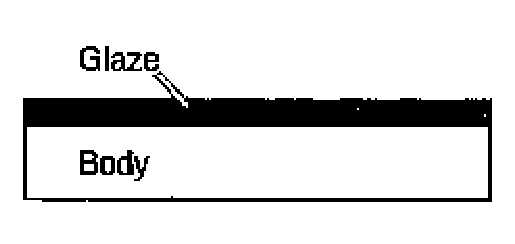
\includegraphics[width=0.6\linewidth]{img/coesame.eps}
  \caption{The body and glaze have the same coefficient of expansion.}
  \label{fig:coesame}
\end{figure}
%-------------------------------------------------------------------------------
Figure~\ref{fig:coeglaze} shows a glaze that has a higher coefficient of 
expansion (CoE) than the body.
%-------------------------------------------------------------------------------
\begin{figure}[htbp!]
  \centering
  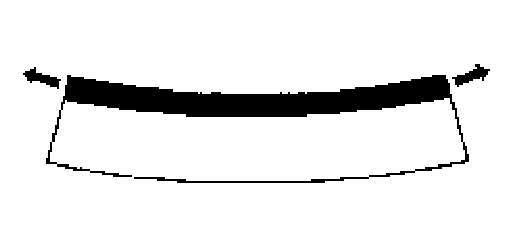
\includegraphics[width=0.6\linewidth]{img/coeglaze.eps}
  \caption{The glaze has a higher coefficient of expansion than the glaze.}
  \label{fig:coeglaze}
\end{figure}
%-------------------------------------------------------------------------------
The glaze contracted more, so it is shorter and therefore the glaze is under a 
tensile stress (it is pulled apart). If the body is very thin it will bend as 
shown. The arrows in figure~\ref{fig:coearrow} show the direction of the stress 
the glaze is under.
%-------------------------------------------------------------------------------
\begin{figure}[htbp!]
  \centering
  
\includegraphics[width=0.6\linewidth]{img/coearrow.eps}
  \caption{Arrows show the tensile stress of a glaze which has a higher 
  coefficient of expansion than the glaze.}
  \label{fig:coearrow}
\end{figure}
%-------------------------------------------------------------------------------
More often the tensile stress is relieved by cracks in the glaze as shown in 
this figure. This is called crazing. The stress caused by high CoE of the glaze 
may be relieved by crazing as soon as the pot is taken out of the kiln or it 
may take days, months or years. The longer it takes, the closer is the CoE of 
body and glaze.
%-------------------------------------------------------------------------------
\begin{figure}[htbp!]
  \centering
  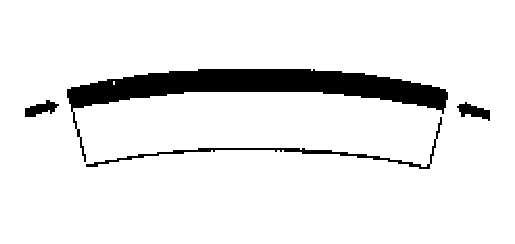
\includegraphics[width=0.6\linewidth]{img/coebody.eps}
  \caption{The body has a higher coefficient of expansion than the glaze.}
  \label{fig:coebody}
\end{figure}
%-------------------------------------------------------------------------------
Figure~\ref{fig:coebody} shows a body with higher CoE than the glaze. The body 
contracted more than the glaze. The glaze is under compression, and if the clay 
is thin it may bend as shown to relieve the pressure. If body contraction is 
only slightly greater than glaze contraction, nothing will happen as shown in 
figure~\ref{fig:coebodynothing}.
%-------------------------------------------------------------------------------
\begin{figure}[htbp!]
  \centering
  
\includegraphics[width=0.6\linewidth]{img/coebodynothing.eps}
  \caption{The body has a higher coefficient of expansion, but because the body 
  contraction is only slightly greater than the glaze contraction nothing 
  happens.}
  \label{fig:coebodynothing}
5\end{figure}
%-------------------------------------------------------------------------------
If a glaze contracts much less than the body, the compression on the glaze 
becomes too much and the glaze will start to flake off (shiver) as shown in 
figure~\ref{fig:coeshiver}. This may not happen by itself, but only if 
something hits the pot. Typically, the rim of a cup will easily chip off.
%-------------------------------------------------------------------------------
\begin{figure}[htbp!]
  \centering
  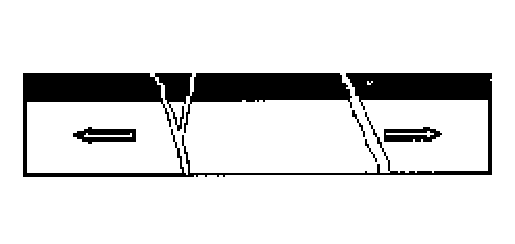
\includegraphics[width=0.6\linewidth]{img/coeshiver.eps}
  \caption{The compression on the glaze is too much and it flakes off.}
  \label{fig:coeshiver}
\end{figure}
%-------------------------------------------------------------------------------
High compression of the glaze may also be relieved by cracking of the body.
%-------------------------------------------------------------------------------
\subsubsection{Moisture Swelling}
When the body has been exposed to humidity for a long period, water enters the 
body, which expands slightly (moisture swelling). This expansion causes the 
glaze to go into tension and it will craze. This kind of crazing is called 
delayed crazing.
%-------------------------------------------------------------------------------
\subsubsection{Solutions}
As we saw above, crazing and shivering are caused by different rates of 
contraction and expansion (different CoE's). The problems are cured by 
adjusting the CoE of body and glaze, so that the two contract and expand more 
closely. It is best if the glaze is left under slight compression.
%------------------------------------------------------------------------------
\subsubsection{Coefficient of expansion}
Ceramic materials have different coefficients of expansion (CoE). 
Table~\ref{tab:coerelative} shows the relative values for the most common.
%------------------------------------------------------------------------------
\begin{center}
  \renewcommand{\arraystretch}{1.5}
  \begin{table}\centering
    \begin{tabular}{|c|c|}\hline
      \textbf{Material}&\textbf{Relative CoE}\\\hline\hline
      %------------------------------------------------------------------------------
      \ce{Na2O}&High\\\hline
      %------------------------------------------------------------------------------
      \ce{K2O}&-\\\hline
      %------------------------------------------------------------------------------
      \ce{CaO}&-\\\hline
      %------------------------------------------------------------------------------
      \ce{BaO}&-\\\hline
      %------------------------------------------------------------------------------
      \ce{TiO2}&-\\\hline
      %------------------------------------------------------------------------------
      \ce{Fe2O3}&-\\\hline
      %------------------------------------------------------------------------------
      \ce{Al2O3}&-\\\hline
      %------------------------------------------------------------------------------
      \ce{PbO}&-\\\hline
      %------------------------------------------------------------------------------
      \ce{CuO}&-\\\hline
      %------------------------------------------------------------------------------
      \ce{MnO}&-\\\hline
      %------------------------------------------------------------------------------
      \ce{ZrO2}&-\\\hline
      %------------------------------------------------------------------------------
      \ce{SnO2}&-\\\hline
      %------------------------------------------------------------------------------
      \ce{P2O5}&-\\\hline
      %------------------------------------------------------------------------------
      \ce{ZnO}&-\\\hline
      %------------------------------------------------------------------------------
      \ce{MgO}&-\\\hline
      %------------------------------------------------------------------------------
      \ce{SiO2}&-\\\hline
      %------------------------------------------------------------------------------
      \ce{B2O3}&Low\\\hline
%------------------------------------------------------------------------------ 
   \end{tabular}
    \caption{Relative coefficient-of-expansion values for common ceramic 
    materials.}
    \label{tab:coerelative}
  \end{table}
\end{center}
%------------------------------------------------------------------------------
\subsubsection{Adjusting the coefficient of expansion of a glaze}
From this list we can see that if we replace soda (\ce{Na2O}) with boron 
(\ce{B2O3}) in a glaze we will lower the CoE of the whole glaze. This can be 
done without changing the melting point of the glaze. Addition of silica will 
lower the glaze's CoE but will also raise its melting point.

If shivering occurs, it means the CoE of the glaze is too low. Adjusting it 
means adding soda (\ce{Na2O}) and reducing boron (\ce{B2O3}).
%-------------------------------------------------------------------------------
\subsubsection{Adjusting the coefficient of expansion of a body}
Adjustment of body CoE is not done according to the CoE of the materials listed 
above. The contraction rate of the body depends to a much higher degree on the 
sudden reversible contraction of silica crystals when these change their 
crystal structure (cristobalite).
%-------------------------------------------------------------------------------
\subsubsection{Quartz change}
Quartz is a crystal form of silica. Quartz is created in the body during firing 
when the clay crystal changes form and releases some of its silica. When quartz 
is heated it changes its crystal structure at 573\degree C. This happens very 
suddenly and is accompanied by a 1\% expansion. On cooling to below 573\degree 
C it contracts again. See figure~\ref{fig:quartzinversion} for a visual 
depiction of this change.
%-------------------------------------------------------------------------------
\begin{figure}[htbp!]
  \centering
  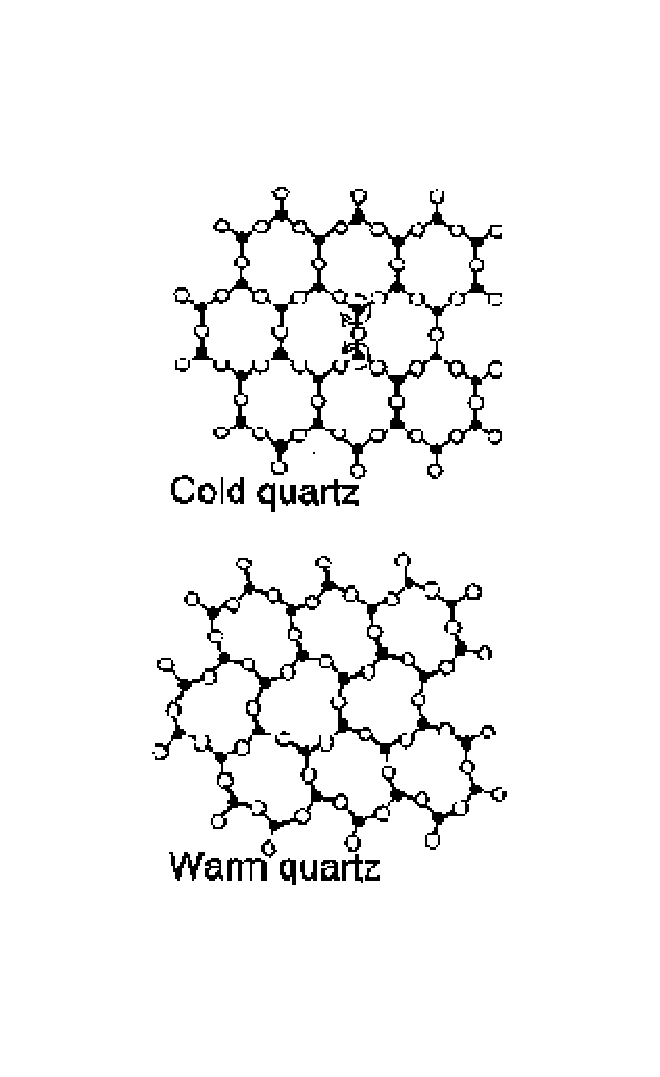
\includegraphics[width=0.6\linewidth]{img/quartzinversion.eps}
  \caption{The volume change of quartz is caused by a rearrangement of the bond 
  between the atoms. At 573\degree C the angle suddenly shifts as shown.}
  \label{fig:quartzinversion}
\end{figure}
%-------------------------------------------------------------------------------
\subsubsection{Cristobalite}
Cristobalite is another crystal form of silica. It changes its size around 
220\degree C and the volume change is nearly 3\%. Cristobalite is created at 
temperatures above 900\degree C from silica released from the clay 
(\ce{Al2O3*2SiO2}) or talc (\ce{3MgO*4SiO2}) or from quartz.
%-------------------------------------------------------------------------------
\begin{figure}[htbp!]
  \centering
  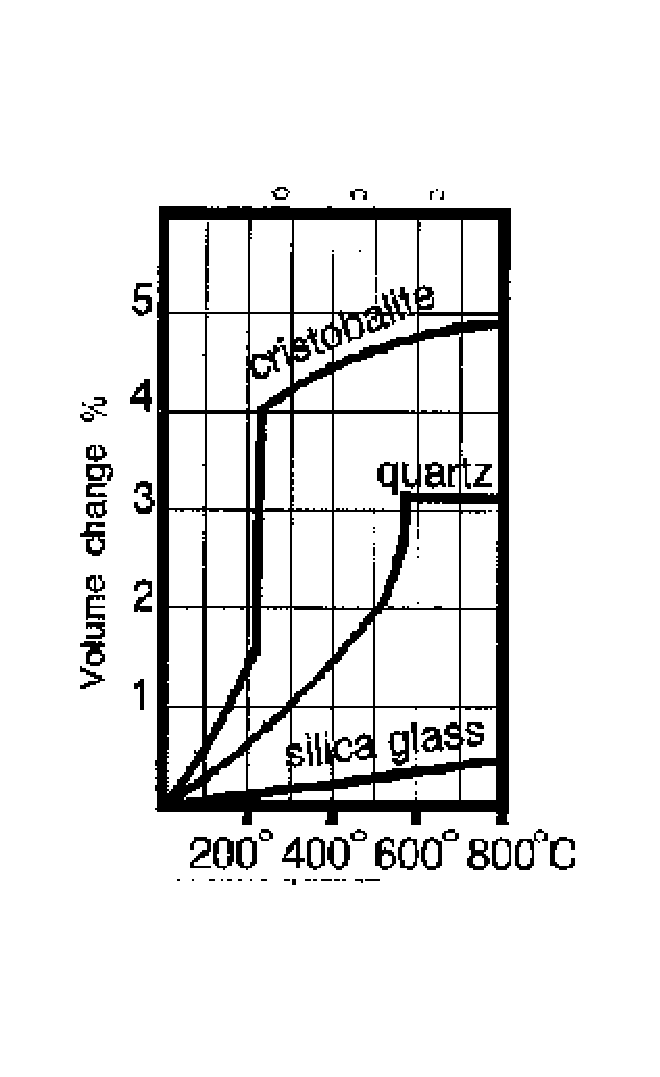
\includegraphics[width=0.6\linewidth]{img/cristobalite.eps}
  \caption{The graph shows volume changes of three forms of silica. The two 
  crystal forms change dramatically but silica in glass hardly changes.}
  \label{fig:cristobalite}
\end{figure}
%-------------------------------------------------------------------------------
\subsubsection{Body-glaze contraction}
The two graphs below show how the body and its glaze contract during cooling. 
The graph in figure~\ref{fig:bodyglazewithout} shows a body that does 
not contain any cristobalite. At 573\degree C the body contracts suddenly due 
to the contraction of quartz, but at this temperature the glaze is still fluid 
enough to follow the contraction of the body.

Around 500\degree C the earthenware glaze hardens and from then onwards 
contracts according to its own CoE. In this example the glaze has a higher CoE 
than the body; it contracts more. This leaves the glaze under tensile stress; 
the glaze is smaller than the body. This will cause the glaze to craze.

The graph in figure~\ref{fig:bodyglazewith} shows contraction of a body 
containing cristobalite. As above, the glaze first follows the quartz 
contraction, then hardens and starts to contract more than the body. However, 
at 220\degree C the cristobalite change causes the body to contract, and at 
this 
temperature the glaze is hard so it is left under compression. This compression 
will prevent the glaze from crazing.
%-------------------------------------------------------------------------------
\begin{figure}[htbp!]
  \centering
  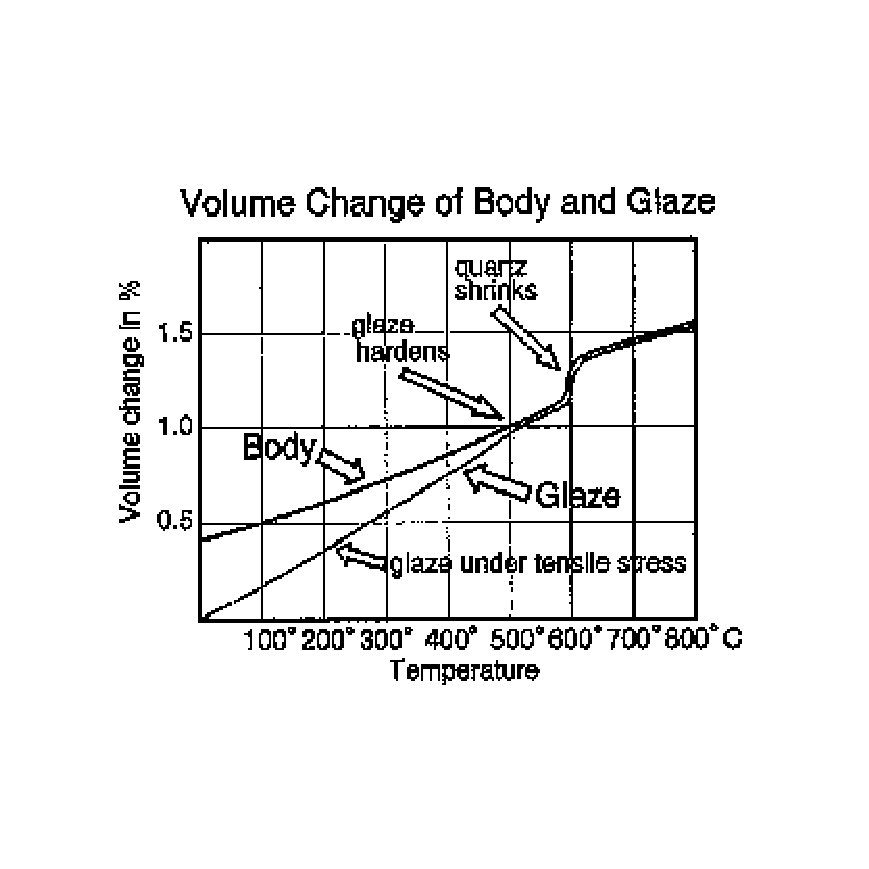
\includegraphics[width=0.6\linewidth]{img/bodyglazewithout.eps}
  \caption{Contraction of body and glaze during cooling. The glaze contracts 
  more 
  so it will craze.}
  \label{fig:bodyglazewithout}
\end{figure}
%-------------------------------------------------------------------------------
\begin{figure}[htbp!]
  \centering
  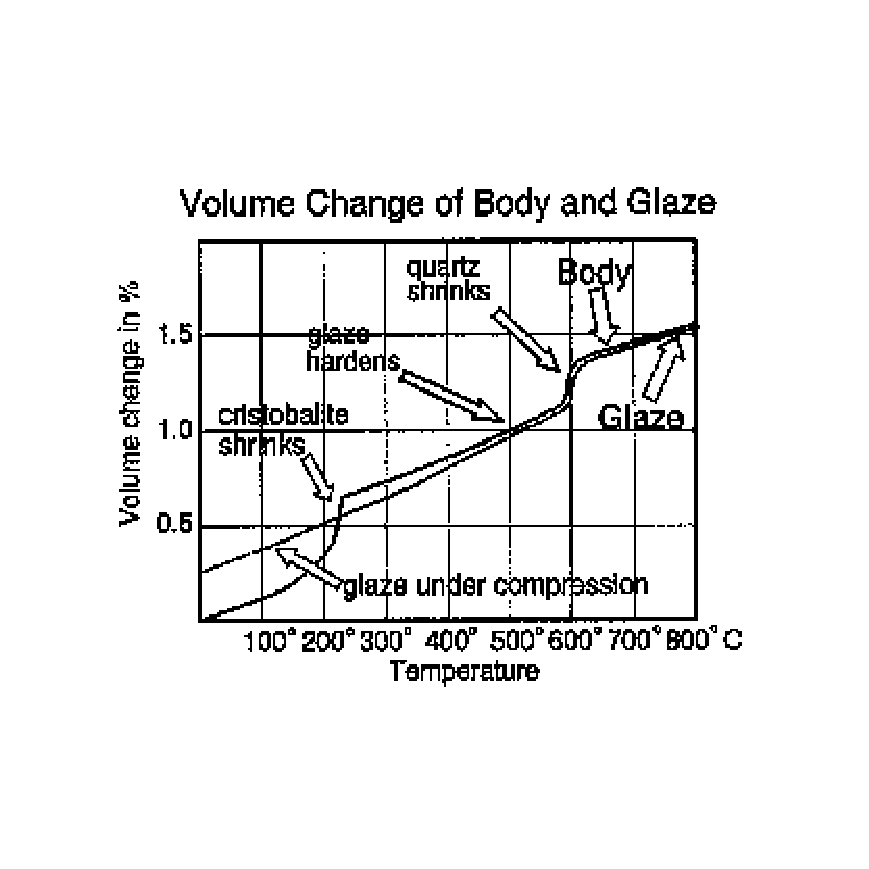
\includegraphics[width=0.6\linewidth]{img/bodyglazewith.eps}
  \caption{The body in this graph contains crisotobalite and shows a sudden 
  contraction at 220\degree C. This causes an overall higher contraction of 
  body compared to glaze.}
  \label{fig:bodyglazewith}
\end{figure}
%-------------------------------------------------------------------------------
\subsubsection{Moisture crazing}
After firing, the porous earthenware body will absorb moisture and this causes 
the body to expand. If the glaze is not under sufficient compression it will 
craze. Such delayed crazing may occur a long time after firing. The moisture 
expansion of the body is reduced by making the body more vitreous. Additions of 
talc or limestone to the body reduce moisture crazing.
%-------------------------------------------------------------------------------
\subsubsection{Crazing cure}
For both types of crazing the cure is:
%-------------------------------------------------------------------------------
\begin{itemize}
\item Add quartz (or silica), talc or limestone to the body.
\item Biscuit-fire to a higher temperature.
\item Glaze-fire to a higher temperature.
\item Add silica to the glaze.
\item In the glaze, replace fluxes with high thermal expansion, like soda 
(\ce{Na2O}) and potash (\ce{K2O}), with boron oxide (\ce{B2O3}).
\end{itemize}
It may seem strange that the cure for crazing is to add silica to both body and 
glaze. The reason is that adding silica to glaze makes it contract less, but 
silica added to the body causes the body to contract more.
%-------------------------------------------------------------------------------
\subsubsection{Crazing test}
There are several ways to test how the expansion of glaze and body fit each 
other. The most simple ones are:
%-------------------------------------------------------------------------------
\begin{itemize}
\item Rings of clay with a diameter of 5 to 10 cm are made with a small gap and 
biscuit. The gap is measured, the ring is glazed on its outer surface and 
refired. After firing the gap is measured to see if the ring has contracted or 
expanded. If the gap has become greater the glaze will craze.
\item Glazed samples are exposed to thermal shocks by repeated heating and 
cooling.
\end{itemize}
%-------------------------------------------------------------------------------
The thermal shocks can be from boiling water into ice water. The number of 
cycles the sample can withstand before crazing indicates its craze resistance.

Another method is to heat the sample at first to 100\degree C then cool it in 
20\degree C water. This is repeated while raising the temperature in steps of 
10 or 20 degrees. The higher the heating temperature the sample withstands 
without crazing the longer it will be able to stay craze-free under normal 
conditions.

A rough guide is:
%-------------------------------------------------------------------------------
\begin{itemize}
\item 120\degree C: craze-free for 8 days
\item 150\degree C: craze-free for 100 days
\item 180\degree C: craze-free for 2 years
\item 200\degree C: craze-free for life
\end{itemize}
%-------------------------------------------------------------------------------
Even if a sample survives the thermal shock test it may still craze due to 
moisture swelling. This can be tested in an autoclave which is simply a 
pressure cooker that can withstand higher pressures. A pressure cooker can be 
used instead. The glaze sample is placed in the pressure cooker with some 
water. It is kept under pressure for a period and then checked for crazing. The 
time it can withstand pressure without crazing indicates the time it may stay 
craze-free under normal circumstances. 

Table~\ref{tab:autoclave} is a rough guide for testing in an autoclave under a 
pressure of 3 atmospheres (about 3 bars). If using a pressure with, say, a 
pressure of 1.5 atmospheres the testing time in the table should be doubled.

All the tests provide only a rough indication of craze resistance. When you do 
the test you will develop your own procedure' which then should always be 
followed faithfully. In this way you will be able to compare your crazing test 
with your previous results.
%------------------------------------------------------------------------------
\begin{center}
  \renewcommand{\arraystretch}{1.5}
  \begin{table}\centering
    \begin{tabular}{|c|c|}\hline
      \textbf{Hours in autoclave}&\textbf{Expected craze-free 
      life}\\\hline\hline
      %------------------------------------------------------------------------------
      1&1--2 years\\\hline
      %-----------------------------------------------------------------------------
      2&2--3 years\\\hline
 %-----------------------------------------------------------------------------
      3&4--6 years\\\hline
%-----------------------------------------------------------------------------
      4&9--10 years\\\hline
%-----------------------------------------------------------------------------
      5&13--15 years\\\hline
%-----------------------------------------------------------------------------
    \end{tabular}
    \caption{A rough guide to testing for crazing in an autoclave.}
    \label{tab:autoclave}
  \end{table}
\end{center}
%-------------------------------------------------------------------------------
\subsection{Crawling}
Crawling appears as areas of clay that are not covered by the glaze. It may be 
small areas or, in extreme cases, the glaze may pull up into a pattern of small 
balls or islands, leaving bare clay in between.

Crawling is caused by:
%-------------------------------------------------------------------------------
\begin{itemize}
\item Poor adhesion of glaze:

Dusty or oily biscuit prevents the glaze from sticking to the body. Refractory 
oxides (chrome, rutile) or underglazes that act as a dust layer prevent the 
formation of an interface. Adding clay, borax or frit to the underglaze 
colorants helps.

\item High surface tension:

High surface tension of the glaze in melting pulls it into islands before the 
clay/glaze interface forms. This is caused by certain oxides, especially 
magnesia, clay and zinc oxide. The solution is to replace magnesia by other 
materials, to calcine part of the clay or to use calcined zinc oxide instead of 
raw.

\item Cracking of glaze layer:

Extensive shrinkage of glaze in drying and early stages of firing, usually 
caused by too much clay content or by overgrinding the glaze, causes the glaze 
to crack and separate from the body. A thick glaze layer is more likely to 
crack.
\end{itemize}
%-------------------------------------------------------------------------------
\subsection{Pinholing and Blistering}
Pinholes appear as tiny holes in the glaze surface. Blisters look like frozen 
bubbles or craters. They are a problem in utilitarian ware, as they collect 
dirt. They may be only on the surface of the glaze or may penetrate to the clay 
layer.

During firing gas bubbles are formed in the melted glaze. The bubbles will move 
to the surface of the fluid glaze and be released.

If you watch any glaze melting, you can actually see this process. Some glazes 
(especially those containing raw borax) foam and boil until they finally smooth 
out. When the firing is stopped before the glaze has had time to heal over, a 
pinhole or crater is left (see figure~\ref{fig:pinholing}). Since overfiring 
also causes pinholes it is better to keep the maximum temperature for some time 
(soaking period).

%-------------------------------------------------------------------------------
\begin{figure}[htbp!]
  \centering
  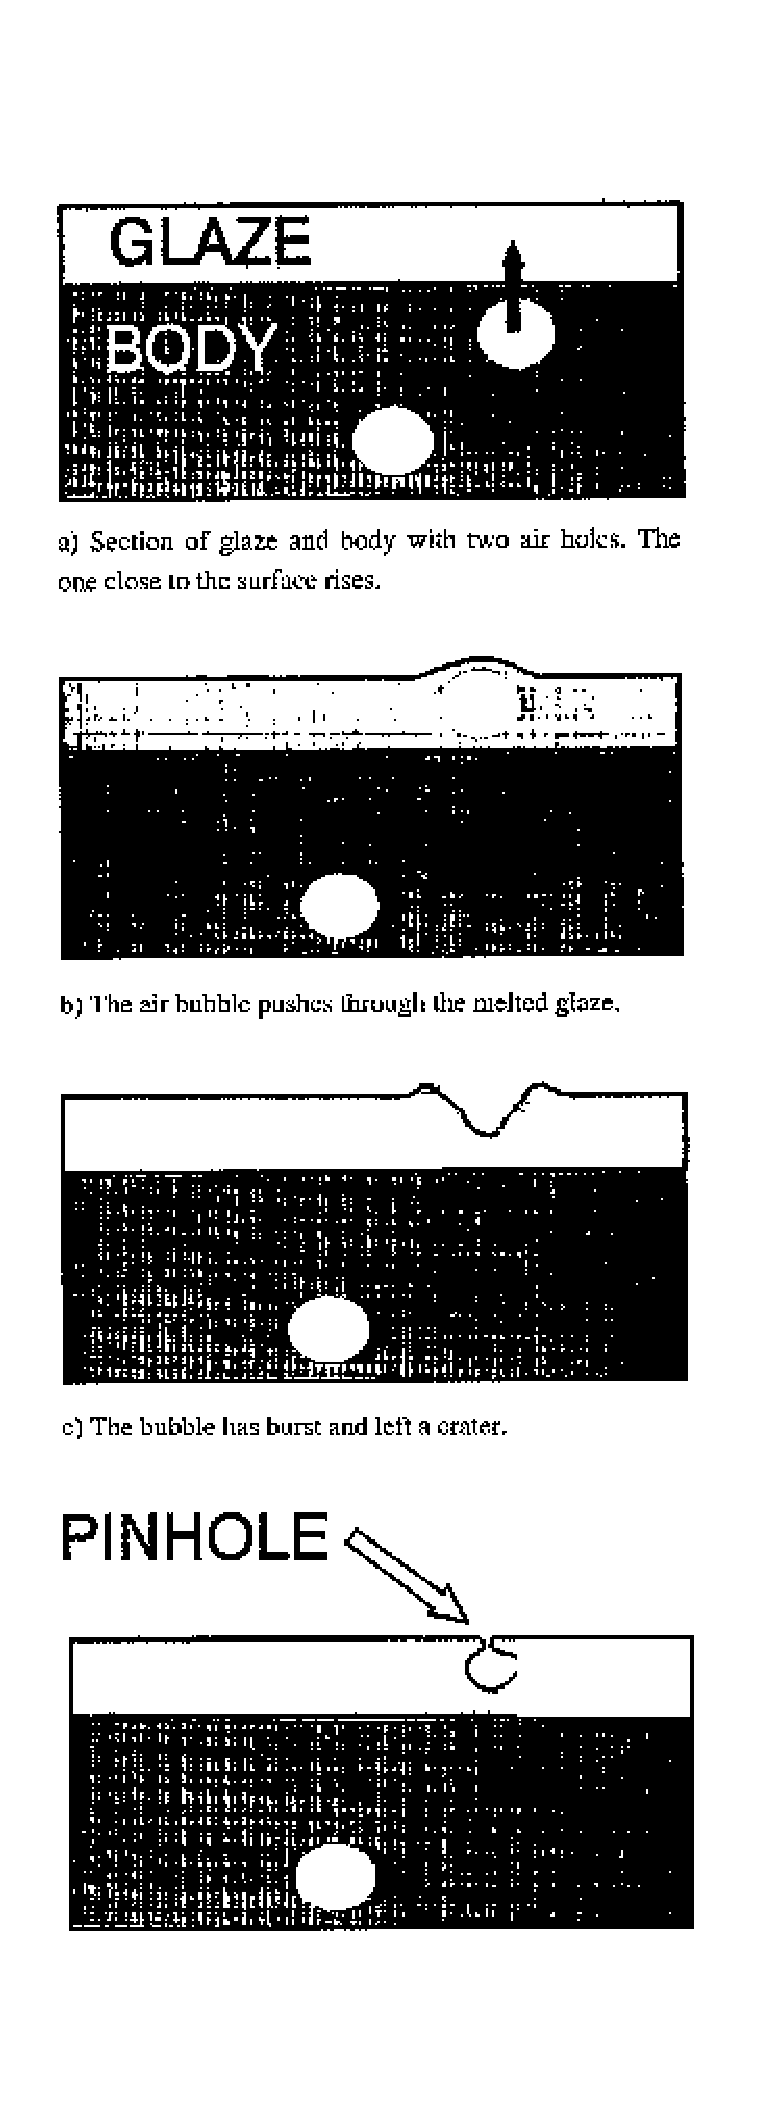
\includegraphics[width=0.6\linewidth]{img/pinholing.eps}
  \caption{How pinholes form in a glaze.}
  \label{fig:pinholing}
\end{figure}
%-------------------------------------------------------------------------------
The main sources of the gas are:
%-------------------------------------------------------------------------------
\begin{itemize}
\item After glazing, a large volume of air exists in the space between the 
solid glaze materials. The air gathers into bubbles during sintering and 
melting.
\item Release of sulfates and carbon in the body and from some of the glaze 
materials.
\item Air bubbles in the body introduced by improper handling of the casting 
slip.
\item Sulfates and carbon from the fuel may deposit in the body during the 
initial stages of firing. Above 900\degree C the gas will be released.
\end{itemize}
%-------------------------------------------------------------------------------
It is important to find out if the problem is in the glaze or in the body. 
Relatively large pinholes that go all the way to the body are usually caused by 
small holes in the body that do not accept the glaze-this is most common with 
slip-cast ware, or with common red clay that contains particles of organic 
matter, sand or mica.

Problems arise if the glaze starts to cool and solidify while bubbles or 
craters are still forming.

Detailed causes and solutions are given in section~\ref{sec:problemmelt}.
%-------------------------------------------------------------------------------
\subsection{Color Changes}
Potters are often plagued by changes in glaze color, either within the same 
kiln-load or from separate firings.

Often this problem can be traced to glaze preparation. The colors may not be 
ground finely enough, weighing may be incorrect, raw materials may have changed.

Otherwise, the problem usually is due to more or less reduction than usual. 
This is one of the most difficult conditions to control in firing and depends 
completely on the skill of the firemaster.

The problem is worst in glazes that contain color oxides that are sensitive to 
reduction. The most sensitive is copper, which is green in oxidation and red in 
reduction; and iron oxide, which is yellow, red to brown in oxidation and 
mottled red-brown, grey to blue or green in reduction. Other oxides change less.

Heavy reduction will darken the iron in the body, which will affect the glaze, 
also darkening it. Sometimes a pot will be dark on the reduced side and light 
on the oxidized side.

Other causes and solutions are given above.
%-------------------------------------------------------------------------------